\documentclass[11pt,twoside,english]{article}
\usepackage{times}
\usepackage[T1]{fontenc}
\pagestyle{headings}

\usepackage{graphicx}
\usepackage{hyperref}
\usepackage{listings}
\usepackage{multicol}

\setlength\parskip{\medskipamount}
\setlength\parindent{0pt}

\renewcommand\textfraction{0.05}
\renewcommand\floatpagefraction{0.95}
\renewcommand\topfraction{0.8}
\renewcommand\bottomfraction{0.8}

\makeatletter


%%%%%%%%%%%%%%%%%%%%%%%%%%%%%% User specified LaTeX commands.

 \setlength{\textwidth}{155mm}
 \setlength{\oddsidemargin}{0mm}
 \setlength{\evensidemargin}{0mm}

\pagestyle{myheadings}
\markboth{GRAFFER}{Version 4.13}

%\usepackage{babel}
\makeatother
\begin{document}


\title{
\includegraphics[width=0.80\textwidth]{logo} \\
  A Flexible Electronic Graph Paper\\
  Version 4.08 (Fortran)\\
  User's Guide}

\author{\textsf{\textbf{\Large James Tappin}}\\
  \texttt{\textbf{\Large jtappin at gmail dot com}}}

\date{\textsf{\textbf{\large June 2020}}}

\maketitle

\begin{multicols}{2}
  \tableofcontents{}
\end{multicols}

\section{Introduction}


\subsection{What is it?}

The first question to be addressed is {}``What is GRAFFER?''.

The original GRAFFER is a package of IDL routines for generating and
editing plots of data and/or functions. The primary purpose is the
generation of X-Y plots, but as of version 2 there was limited support
for displaying 2-D datasets as contours or in an {}``image'' format,
this support was much improved in 3.x versions and later. The
Fortran version replaces the core interactive plotting program with a
version written in Fortran and using the gtk-fortran and plplot
libraries. 

The plot editing is controlled via a Graphical User Interface (GUI)
which allows you to change scalings, annotations etc. and to add \&
delete traces and even to edit the actual data. Hard copies can be
generated and spooled. The whole plot can then be saved in a GRAFFER
file for future editing.

GRAFFER is not and does not pretend to be a fully-fledged drawing tool
(there are plenty of those around e.g. \texttt{xfig} or commercial
products) but rather tries to do the things that they (well
\texttt{xfig} at any rate) don't do well i.e.\ plotting data.


\subsection{Why is it?}

The earliest versions of GRAFFER were developed in the mid 1990's for
my own use as a consequence of the amount of time I was wasting
adjusting the format of plots to go into papers (e.g. redoing plots
with log axes or with different ranges). Naturally being of a tinkering
turn of mind I gradually added features until GRAFFER became a
reasonably general data-plotting tool.

At about that time a user posted an enquiry to the UseNet group
\texttt{comp.lang.idl-pvwave} as to whether there was a widget-based
graph plotting tool in IDL\footnote{This was well before
  \texttt{iTools}, or even \texttt{Live\_Tools}
  existed.}\footnote{Unfortunately I don't have a record of who it
  was.}. As a result of this GRAFFER version 1.03 was released to the
world.

Since the free IDL clone GDL (GNU Data Language,
\url{http://gnudatalanguage.sourceforge.net/}) still has only limited 
support for widgets, GRAFFER in its original form is limted to those
users with access to the commercial IDL package. For that reason, when
GTK-Fortran became a viable package, I decided to port the core of
GRAFFER to Fortran (using GDL to evaluate functions and for some
utility operations).

\subsection{Requirements}

The Fortran version of GRAFFER requires the gtk-fortran
(\url{https://github.com/vmagnin/gtk-fortran}) and plplot
(\url{http://plplot.sourceforge.net/}) and their dependencies. In
addition, you will need a working Fortran compiler (with a fully
functional \texttt{iso\_c\_binding} module); for \texttt{gfortran},
this means at least version 4.6.0. In addition \texttt{cmake} is
required to build the program.

\subsection{Copyright etc.}

GRAFFER and its component routines may be freely used, copied \&
distributed under the terms of the GNU General Public Licence V3.

\section{Main features}

In this section some of the principal features of GRAFFER are listed.

\begin{itemize}
\item Plot a arbitrary number of X-Y plots on a single set of axes
  (there may be two alternate Y scales).
\item Data for each plot can be:
  \begin{itemize}
  \item Read from a file
  \item Entered with a data editor
  \item Entered with the mouse
  \end{itemize}
\item Functions can be plotted, including doing basic fits to existing
  data plots.
\item Contour or ``image'' display of Z vs. X \& Y (data or function).
\item Easy to change plot limits, log/linear scaling and other axis
  options.
\item Time labelling of axes.
\item A secondary Y-axis may be used to allow the overlay of plots with
  substantially different scales but the same independent variable.
\item Wide range of display styles for individual traces.
\item Generate Postscript, PDF or EPS version of plot.
\item Combining or re-ordering of traces within GRAFFER.
\item All possible combinations of error bars and limits are available.
\item Save plot to a file for future additions or modification.
\item Add a key or legend.
\item IDL/GDL routines exist to add datasets programattically to a
  GRAFFER file.
\end{itemize}


\part{The Main Program}
\label{part:main}


\section{Getting Started}


\subsection{Making sure it's there}

The Fortran version of GRAFFER is an executable that should be placed
in your \texttt{PATH}. Scripts to initialize the supporting gdl/idl
programs are in the \texttt{share/graffer} subdirectory of the
installation prefix. These can be sourced in your \texttt{.bashrc} or
\texttt{.cshrc} file, e.g.
\begin{verbatim}
source /usr/local/share/graffer/graffer_gdl_init.csh
\end{verbatim}
for a C-shell variant, or
\begin{verbatim}
. /usr/local/share/graffer/graffer_gdl_init.sh
\end{verbatim}
for a Bourne shell variant. This will add the path to the GRAFFER
gdl/idl routines to the \texttt{GDL\_PATH} and \texttt{IDL\_PATH}
environment variables.

\subsection{Invoking it}

If GRAFFER is properly installed and its installation directory is in
your path, it can be started simply by typing:
\begin{verbatim}
graffer
\end{verbatim}
at the command prompt. If a filename is given, then that file is opened
or initialized as a new GRAFFER file. If no filename is given, then a
file selector dialogue will be presented to select a file.

Also if your desktop environment supports \texttt{.desktop} files it
may be started from the \texttt{Applications->Education->Science} menu,
and if you define a new mime type for \texttt{*.grf} files, then that
can be bound to the application.

\subsubsection{Environment}
\label{sec:env}

The command to invoke \texttt{gdl} or \texttt{idl} may be specified by
the environment variable \texttt{GRAFFER\_GDL}. This has a lower
priority than a value set in the resource file or the command line
options, but higher than searching in \texttt{\$PATH}. It's probably
not that useful now that the command can be set in the resource file or
on the command line.

\subsubsection{Keywords}

GRAFFER can accept a number of keywords to control its operation:

\begin{description}

\item [\texttt{-{}-geometry} or \texttt{-g}:] Specify a geometry for the
  drawing window in the form \textit{x}\texttt{x}\textit{y} (e.g.\
  \texttt{-{}-geometry=800x800}). The default is \texttt{600x600}.
\item[\texttt{-{}-mouse} or \texttt{-m}:] Allow interactive editing of
  new datasets  by default. May be negated as \texttt{-{}-nomouse} to
  override a setting in the resource file.
\item[\texttt{-{}-suppress\-2d} or \texttt{-s2}:] Suppress the display
  of 2D datasets. Can be useful on a slow machine. May be negated to
  override a setting in the resource file.
\item[\texttt{-{}-delete} or \texttt{-d}:] Delete program and data
  files generated by function evaluation. May be negated to override
  a setting in  the resource file.
\item[\texttt{-{}-pdf} or \texttt{-p}:] Set a viewer for the PDF help
  files (e.g. \texttt{-{}-pdf okular}).
\item[\texttt{-{}-autosave} or \texttt{-a}:] Set the delay between
  autosaves in seconds (e.g. \texttt{--autosave 180}) Default is 300.
\item[\texttt{-{}-colour-table} or \texttt{-ct}:] Specify the name stem
  of the colour table files (e.g. \texttt{-{}-colour-table my\_tables})
  Default is \texttt{c\_tables}.
\item[\texttt{-{}-colour-dir} or \texttt{-cd}:] Specify the directory
  with the colour table files (e.g. \texttt{-{}-colour-dir ./data}
  Default is to check in \texttt{/usr/local/share/graffer} and
  \texttt{/usr/share/graffer}. 
\item[\texttt{-{}-gdl} or \texttt{-{}-idl}:]
  Specify the command to run GDL or IDL to evaluate functions
  (e.g. \texttt{--gdl /usr/local/bin/gdl-git}). Default it to try first
  the \texttt{GRAFFER\_GDL} environment variable then to try first
  \texttt{gdl} and then \texttt{idl} in the user's path.
\end{description}

\subsection{A quick tour of the main window}

\begin{figure}[htbp]
  \centering
  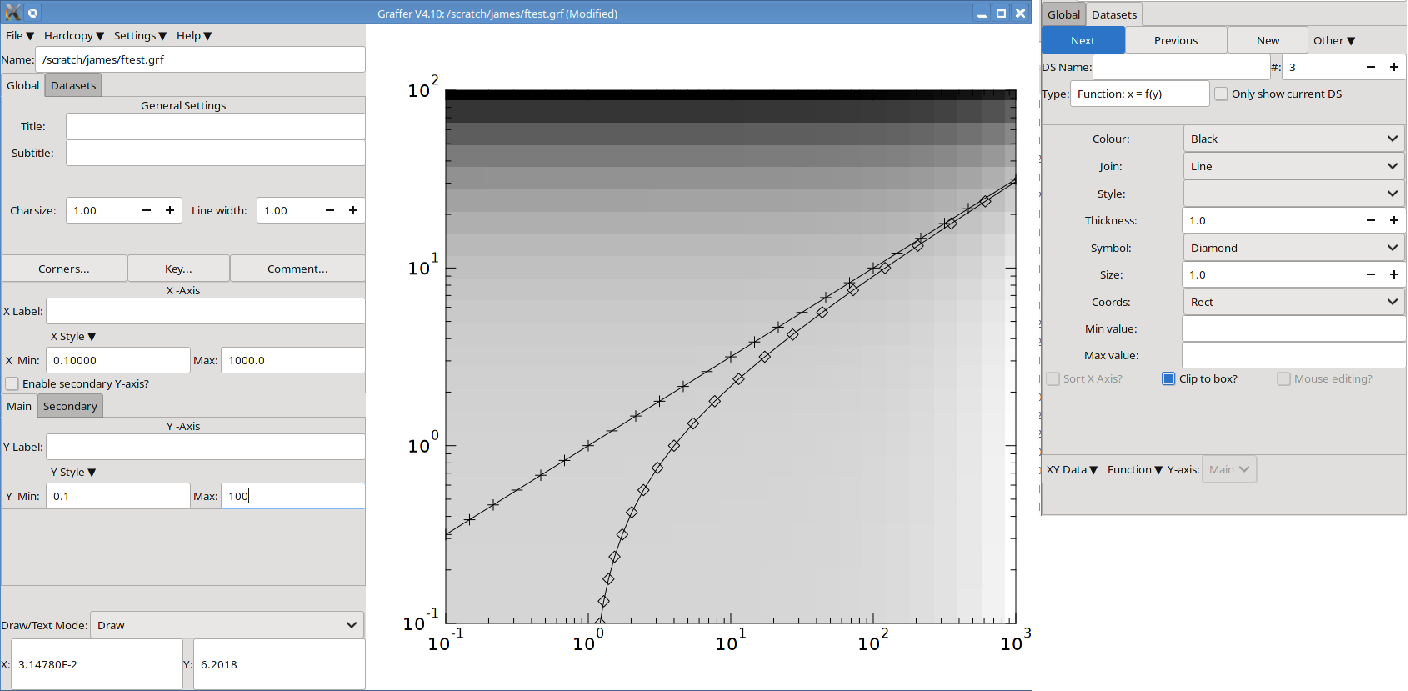
\includegraphics[width=\textwidth]{Main}
  \caption{The layout of the main GRAFFER window. (With the dataset tab
    shown to the right).}
  \label{fig:main}
\end{figure}
Now that you've got GRAFFER running and a file selected, you should see
the main GRAFFER window. Depending on which mode you are operating in,
it should look like \textsc{\autoref{fig:main}}.  The main areas of the
window are:

\begin{description}
\item [Main~plotting~window:]This is where the plot is drawn. For
  suitable datasets you can operate on the data using the mouse in the
  plotting window.
\item [Utility~control~menu:]This is at the top of the control panel
  and contains the buttons for exiting GRAFFER, saving the file,
  printing it, opening new files etc. Immediately below it is a box
  that displays the current file and directory, this cannot be changed
  by the user.
\item [General~settings:]The settings which apply to the whole plot
  (title, positioning etc) are set from the {}``General settings'' box,
  which is just below the utility controls.
\item [Axis~settings:]The two axis settings boxes allow you to set the
  properties of the individual axes. There is one for the X and one for
  the Y axis. The secondary Y-axis is enabled by the checkbox button,
  and the settings for it are in the secondary tab.
\item [Dataset~control:]In the alternate tab (shown separately to the
  right of \textsc{\autoref{fig:main}}) are most of the items which are
  concerned with selecting datasets, loading data and setting the
  format of the trace.

\item[Information boxes] Below the main plot window are two small boxes
  showing the current cursor location when it is inside the plot window.

\end{description}

\section{Datasets}


\subsection{General comments}

The basic element of a GRAFFER plot is the \textsc{dataset}. A dataset
corresponds to a trace on the resulting plot. In the resulting plot all
the datasets are plotted on a single set of axes, using a single
scaling. All data-input and {}``line format'' operations operate on the
\textit{current} dataset.

There are four classes of dataset in GRAFFER, divided into two broad
types each with two sub-classes.


\subsubsection{Observational data }

An observational dataset consists of tabulated numbers which are
entered by the user in one of a number of ways (see below). The
subclasses are:

\begin{description}
\item [X-Y~data:]Also referred to as 1-D data. This is the basic
  GRAFFER dataset and consists of a set of tabulated X \& Y values with
  optional error limits.
\item [Z~data:]Also referred to as 2-D data. This is a rectangular
  array of Z values and the X \& Y values at which they are
  measured. Note that the grid must be rectangular but it need not be
  regular.
\end{description}

\subsubsection{Functions }

A function dataset is an IDL expression which can be evaluated by
GRAFFER. As with observational data, they are divided by
dimensionality. In the Fortran version, these functions are evaluated
by spawning a process running gdl or idl and then reading the resulting
data file.

\begin{description}
\item [1-D~functions:]A 1-D function dataset is an IDL expression which
  when fed an array returns another of the same length. {[}There is
  also a special case of parametric function datasets where two
  expressions are needed.{]}
\item [2-D~functions:]A 2-D function, takes 2 1-D arrays as its input
  and returns a 2-D array.
\end{description}
Note that for any dataset other than the first, the dataset must first
be created see below (p.~\pageref{make-new-ds}).


\subsection{Entering 1-D observational data\label{enter-1d}}

The usual methods of entering observational data are accessed via the
\textsc{X-Y data} pulldown menu.

\begin{table}[!ht]

  \caption{\label{ecodes}\textit{The error-bar codes in dataset files.}}

  \begin{center}
    \begin{tabular}{|l|cccc|c|}
      \hline 
      Code&Col 3&Col 4&Col 5&Col 6&Default?\\
      \hline
      \textit{none} & - & - & - & - & 2 \\
      \#Y&$\pm Y$&-&-&-&3\\
      \#X&$\pm X$&-&-&-&\\
      \#YY&$-Y$&$+Y$&-&-&4\\
      \#XX&$-X$&$+X$&-&-&\\
      \#XY&$\pm X$&$\pm Y$&-&-&\\
      \#XYY&$\pm X$&$-Y$&$+Y$&-&5\\
      \#XXY&$-X$&$+X$&$\pm Y$&-&\\
      \#XXYY&$-X$&$+X$&$-Y$&$+Y$&6\\
      \hline
    \end{tabular}
  \end{center}
\end{table}

\subsubsection{From a File}

First create an ASCII file with one line for each datum with value in
the order:

\begin{verbatim}
  X Y "lower X err" "upper X err" "lower Y err" "upper Y err"
\end{verbatim}
Any or all of the error limits may be omitted. The interpretation of
the error columns is determined by an error-bars code which is a line
starting with a hash (\#) sign and then the appropriate combination of
\texttt{X}'s and \texttt{Y}'s. The possible values are described in
\textsc{\autoref{ecodes}}. The preferred extension of the file name is
\texttt{.dat}.

To read the file, select the {}``\texttt{From file...}'' option of the
{}``\texttt{XY data}'' pulldown. This will generate a file-selector
widget which you can use to select the file. When you have the file you
want, click on the {}``\texttt{OK}'' button.

N.B. If the dataset already contains values these will be
\textbf{replaced}; if the dataset is a function then a warning is
given.


\subsubsection{Via the data editor }

If you have the values on a piece of paper (some of us still
occasionally make measurements manually and write them down in a
notebook), or if you want to remove some bad values from a dataset then
you can use the dataset editor.

The {}``\texttt{Edit values}'' option of the {}``\texttt{XY data}''
pulldown invokes the data editor. This is just an IDL text widget in
which the values in the current dataset are displayed. The normal
selection, cutting etc.\ apply.

Below the editor window is a pulldown to select the error limit
interpretation.  Only those options appropriate to what GRAFFER
\textit{thinks} is the number of columns are actually selectable


\subsubsection{With the mouse}

This method of editing a dataset is potentially dangerous, and is
disabled by default (you can change the default via the
\texttt{Options...} menu option) and can be enabled for individual
datasets via the \texttt{Extras} menu in the dataset tab.  It can
however be useful for removing bad data or for indicating features
displayed in a 2-D dataset.  

The three mouse buttons each have a function (this is where the
assumption that you have a 3-button mouse comes in):

\begin{description}
\item [Left:]Enter a point: for a dataset without errors a point is
  entered at the position of the cursor; for a dataset with errors the
  dataset editor (above) is invoked with the selection point at the end
  of the dataset. The position is set at the \textbf{release} of the
  button. When the button is pressed, if there is already at least one
  point in the dataset then the cross-hairs are replaced by a line
  showing the new segment. 

  If the \textsf{ctrl} key is down when the mouse button is pressed and
  the cursor position is within 5 pixels of a line segment, then the
  point is inserted between the endpoints of that segment (in the
  unlikely event of the point being within 5 pixels of more than one
  segment, then the closest is chosen).

  If the \textsf{shift} key is down when the mouse button is pressed
  then the point will be added at the end of the dataset nearer to the
  cursor location (this allows you to prepend points).

  The point is always placed at the location of the cursor when the
  button is \textbf{released}.

\item [Centre:]Edit a point: for a dataset without errors the point
  nearest to the cursor when the button is pressed is moved to the
  location of the cursor when the button is released; for a dataset
  with errors the dataset editor is invoked with the pointer at the
  point nearest to the cursor. N.B. As a safety precaution, the cursor
  must be within 5 pixels of the point. When the button is pressed then
  the cross-hairs are replaced by a line showing the updated
  segment(s).
\item [Right:]Delete a point: the point nearest the cursor when the
  button is released is deleted.  N.B. As a safety precaution, the
  cursor must be within 5 pixels of the point. A circle is drawn around
  the point to be deleted if one is in range.
\end{description}
If \textsf{ctrl} or \textsf{shift} is held down when the button is
released, then the action will be cancelled. N.B.\ this means that for
inserting or prepending points, you must release the modifier key
before releasing the mouse button.

\subsubsection{A note on limits}

In many situations in the real world, some of the values in a dataset
are upper or lower limits. To plot limits requires that the dataset be
defined with asymmetrical error bars. If the value is a lower limit,
then set the \textbf{upper} error to \texttt{Inf} (The IEEE
$\infty$ value), for an upper limit, set the \textbf{lower} error to
\texttt{Inf}.

\subsubsection{Copying another dataset}
\label{sec:xycopy}

If the \texttt{Copy ...} option is selected, then a menu will give you
a choice of existing XY datasets to copy to the current dataset. By
default if the current dataset contains data, then only those of the
same type are offered, but this can be overridden by selecting the
``Show all'' button. A warning will be given before attempting to
overwrite functions or 2-D data.

This is useful (for example) if you have a dataset that you want to
plot over an image display, and you need black and white dashes to make
it show up; in that case you could set the original to black continuous
and then make a copy and display that with white dashes.


\subsection{Entering 2-D observational data\label{enter-2d}}

The entry of 2-D data is somewhat more restricted that 1-D because:

\begin{enumerate}
\item A dataset editor for 2-D data would be too unwieldy
\item Mouse editing of 2-D data is clearly not feasible.
\end{enumerate}
Therefore there are only two ways to enter 2-D data, all of which are
reached via the \texttt{2-d datasets} sub-pulldown of the \texttt{XY
  data} pulldown.


\subsubsection{From a file}

Again very similar to the 1-D case but the rules for laying out the
file are different in that some {}``header'' information is needed.
The format of the file:

\begin{itemize}
\item Line1: 2 numbers giving the number of X and Y values ($n_{x},\,
  n_{y}$). If $n_x$ is negative, this means the X array is
  2-dimensional, and if $n_y$ is negative then the Y array is
  2-dimensional.
\item The $n_{x}$ or $n_x \times n_y$ X values. These may be spread
  over any number of lines, but there must be the correct number and a
  new-line at the end.
\item The $n_{y}$ or $n_x \times n_y$ Y values. These may be spread
  over any number of lines, but there must be the correct number and a
  new-line at the end.
\item The $n_{x}\times n_{y}$ Z values. Again they may be spread over
  any number of lines, but there must be the correct number of values.
\end{itemize}
Note that there are no error bars on 2-D datasets.

\subsubsection{Copying another dataset.}
\label{sec:zcopy}

Again very similar to the 1-D case. There is however no ``Show all''
button as there is only one type of 2-D dataset.

\subsection{Entering functions\label{enter-fun}}

Although there are several varieties of function in GRAFFER, the format
for expressing them and the editor used to enter them are very similar
for all types. The various function editors are reached via the
\texttt{Function} pulldown which is found adjacent to the \texttt{XY
  data} pulldown.


\subsubsection{The Editors }

The four types of function can all be entered via one of the function
editors. These all share the following fields:

\begin{description}
\item [Function:]A box or boxes in which to enter the function. This
  must be a valid IDL expression which returns an array of the same
  size as its input argument.
\item [Axis~Range:]two or four boxes to enter the limits over which the
  function is to be evaluated. If no values are entered, then the range
  of the axis of the independent variable is used.
\item [Number~of~evaluations:]One or two boxes to the GRAFFER how many
  time to evaluate the function over its range (the default for this is
  25, but for straight lines you only need 2 while very wiggly
  functions may need many more).
\item [Apply~\textmd{and}~Cancel:]Self-explanatory, the \texttt{Apply}
  button accepts the new function definition and the \texttt{Cancel}
  button rejects it.
\end{description}
The precise details vary according to the type of function being
specified:

\begin{description}
\item [\texttt{y~=~f(x):}]This is the obvious type of 1-D function. The
  function entered in the function box should be an IDL expression with
  \texttt{x as} the independent variable e.g.:

\begin{verbatim}
  sin(x)
  3.2{*}x^2 - x + !pi
  replicate(5.1,n_elements(x))
\end{verbatim}
\end{description}
Note that this last case is necessary as the obvious \texttt{5.1} does
not return an array\footnote{I suppose you could use \texttt{{[}5.1,
    5.1{]}} but then if you reset the number of evaluations you'd be up
  a gum tree (at least temporarily).}.

\begin{description}
\item [\texttt{x~=~f(y)}:]Very similar except that now x is expressed
  as a function of y so the independent variable should now be
  \texttt{y} e.g. \texttt{exp(-y\textasciicircum{}2) - 0.5}.
\item [\texttt{x~=f(t)~\&~y~=~g(t)}:]Also referred to as a parametric
  function. There are several important points here:

  \begin{itemize}
  \item There are now two function boxes to be filled, the first gives
    x as a function of t and the second gives y as a function of t. For
    example to draw a unit circle (or part thereof; see below) you
    would need to set the functions as: \texttt{sin(t)} \&
    \texttt{cos(t)}.
  \item The range of evaluation \textbf{must} be given as the parameter
    is not linked to an axis and so there is no natural boundary. The
    default is to go from 0 to 1.
  \end{itemize}
\item [\texttt{z~=~f(x,y)}:]The 2-D function entry. This requires a
  function of both X and Y to be given. Examples would be:

\begin{verbatim}
  x * sin(y)
  -1./sqrt(((x+.5)^2+y^2)>1e-6) - .5/sqrt(((x-1)^2+y^2)>1e-6) - (x^2 + y^2)
\end{verbatim}
\end{description}
In this latter case, note the use of the limiting operators to flatten
out the singularities which will, if they lie at an evaluation point,
cause GRAFFER to crash. Internally, the \texttt{x} and \texttt{y}
arrays are converted into 2-D arrays so that the examples above do
return the proper 2-D array of z-values.

As there are two independent variables, there are two sets of limits
and two evaluation counts. If you are on a system with limited memory,
remember that the function evaluation requires (at least) 3 arrays of
double precision numbers with $N_{x}\times N_{y}$\ points.

\subsubsection{Copying another function}
\label{sec:fcopy}

The \texttt{Copy ...} option allows you to copy an existing function
dataset to the current. As is generally the case a warning is given
before overwriting incompatible datasets. If the current dataset is a
function then by default only functions of the same kind are offered as
candidates, but the ``Show all'' button allows all functions to be
offered.

\subsubsection{Fit dataset }

Often, when you have observational or experimental data, you want to
fit a function to that data. While GRAFFER cannot provide a fully
general function fitting suite, there are facilities to fit polynomials
and other common variations:

\begin{description}
\item [Polynomial:]$y=\sum a_{i}x^{i}$
\item [Exponential:]$y=\exp(\sum a_{i}x^{i})$
\item [Logarithmic:]$y=\sum a_{i}\ln(x)^{i}$
\item [Power~law:]$y=\exp(\sum a_{i}\ln(x)^{i})$
\end{description}
Note that the functional forms do in the case of a first-order fit
reduce to the more usual forms it's just easier to implement them the
way they are given here.

To invoke fitting firstly create a \textbf{new} dataset. Do not under
any circumstances attempt to invoke fitting with the data that you wish
to fit as the current dataset, if you do then the original data will be
destroyed! (In the Fortran version, even if the current dataset is a
fittable dataset it is not offered as a candidate).

When you select the fitting option on the function pulldown, a pop-up
control panel will appear which allows you to select which dataset to
fit and what kind of fit to do.

The default fitting style is a first-order fit which will appears as a
straight line with the current selection of logarithmic and/or linear
axes (e.g. for a log-log plot the default will be a power-law).  The
order of the fit for the {}``conventional'' forms is just the maximum
value of $i$.


The \texttt{update} button allows you to try a fit without destroying
the pop-up. By using this you can try various types of fit and select
the best. Note that the $\chi^{2}$ values quoted are meaningful in an
absolute sense only if the dataset being fitted has error bars, however
even for datasets without errors they do provide a relative measure of
the quality of the fit.


\subsubsection{Read function from file}

There is also an option to read a function from a file. This is most
likely to be used in conjunction with the option to save a dataset to a
file as a means of transferring complicated functions from one GRAFFER
file to another. Lest you should wish to write a function definition
with an editor and then read it into GRAFFER the format is:

\begin{description}
\item [Line~1]A function type code, which gives the \textbf{Dependent}
  variable, i.e. \texttt{Y}$\equiv y=f(x)$, \texttt{X$\equiv x=f(y)$},
  \texttt{XY$\equiv x=f(t),\: y=g(t)$} and \texttt{Z}$\equiv z=f(x,y)$.
\item [Line~2]The range over which the function is to be evaluated: 2
  numbers except for type \texttt{Z} where 4 are needed.
\item [Line~3]The number of function evaluations: 1 number except for
  type \texttt{Z} where 2 are needed.
\item [Line~4]The function itself, type \texttt{XY} needs a fifth line
  with the second function.
\end{description}

\subsection{Dataset selection and manipulation}

In addition to entering datasets, there are several other operations
that need to be performed on them. These {}``selection and
manipulation'' operations are described in the following
paragraphs. The controls for the operations are found at the top of the
\textsf{dataset} tab on the main window.


\subsubsection{Selection}

\begin{description}
\item [Create~new~dataset\label{make-new-ds}:]The \texttt{New} button
  on the dataset operations menu creates a new empty dataset at the end
  of the dataset list into which data or a function can be inserted.
  The same operation can be effected via the \texttt{select} option of
  the \texttt{Other} pulldown and selecting the item \texttt{<new>} in
  the pop-up menu.
\item [Select~dataset:]All operations such as reading data or changing
  linestyles are applied to the \textsc{current} dataset. Therefore you
  need a mechanism whereby you can make a given dataset current.


  The simplest mechanism is via the \texttt{next} and \texttt{previous}
  buttons which allow you cycle through the currently defined datasets.
  This is all very well for GRAFFER files with a handful of datasets,
  but for a file with many datasets (the most you are allowed to have
  is $2^{15}-1$ but I doubt if you will be seriously inconvenienced by
  this limit!) this could be rather time consuming, so there is an
  alternative method: the \texttt{Other} pulldown has an option
  \texttt{Select} which generates a pop-up menu with all the datasets
  listed with their sizes, types and names. To select the required
  dataset, just scroll the list widget (if necessary) and click on the
  line for the dataset you want. The \texttt{Cancel} button
  destroys the pop-up and leaves the selection unchanged.

\item [Name:]Technically this probably belongs under the heading of
  {}``Dataset properties'' but conceptually it is better considered
  here, both because if its use and the location of its entry point.


  A dataset can have a name associated with it. This is an arbitrary
  string which is used for two purposes, firstly to identify the
  current dataset and secondly as a label on any legend or key on the
  plot.  The entry box below the dataset operations menu displays and
  also allows you to edit the name of the current dataset. (The serial
  number in the adjacent box is not editable.)

  The only constraint on the string used for the name is that if you
  intend to add a key to the plot then you need to remember that the
  exclamation mark is an escape character.
\item[\#:] The dataset index number. This is a spin button that can be
  used to select a dataset as well as indicating the current dataset.

\item[Only show current DS:] This toggle allows you to display only the
  current dataset (useful in complex plots). Text strings and the key
  (if one is present) are also suppressed when this is selected. If
  text mode (\textsc{\autoref{sec:text}}) is also selected, then only the
  text strings are displayed. If you try to print while this option is
  enabled, then you will be asked whether to print all the datasets or
  just the current.

\end{description}

\subsubsection{Manipulation}

In addition to the basic input and editor operations described in
\textsc{\autoref{enter-1d}-\autoref{enter-fun}}, there are a number of
operations which work on whole datasets. These operations are all
options of the \texttt{Other} button in the dataset operations menu.

\begin{description}
\item[Rescale:] Shift and/or scale the values in a dataset
  (Figure~\ref{fig:rescale}). Not applicable to functions. 
  \begin{figure}
    \centering
    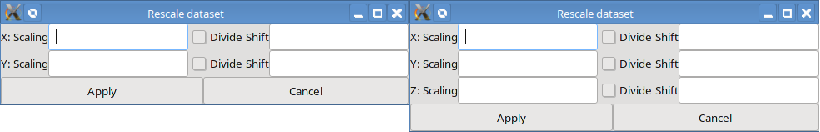
\includegraphics[width=0.75\textwidth]{Rescale}
    \caption{Rescaling menus. Left: 1-D datasets, Right: 2-D datasets.}
    \label{fig:rescale}
  \end{figure}
\item[Transpose:] Exchange the X and Y axes. Not applicable to functions.
\item [Delete:]Delete the current dataset. There is a confirm pop-up
  before the dataset is actually destroyed. The next dataset becomes
  current, unless the dataset deleted was the last in which case the
  previous dataset becomes current.


  You cannot delete the only dataset in a file.

\item [Erase:]Delete the contents of the current dataset but do not
  remove its slot in the GRAFFER file. This can be done to the only
  dataset in a file.
\item [Write~:] Write the current dataset to an ASCII file in a
  format that can be read by the \texttt{Read from file} options of the
  data and function entry menus. A pop-up will appear to allow you to
  specify the filename and directory. If you attempt to overwrite an
  existing file a confirm menu will appear to allow you to {}``back
  out''.
\item[Write as data:] For functions only, evaluate the function and
  write as data.
\item[Copy:] Make a new dataset which is a copy of the current
  dataset. The data values and type are copied. For functions the
  functions and evaluation range are copied. Display properties will be
  the defaults. The new dataset becomes current.
 
\item[Select:] Display a list of datasets, and click on one to make it
  current. 
\item [Sort:]Reorder the datasets. This generates a pop-up that allows
  you to select datasets and move them to a different location in the
  list. This can be useful if you want to make sure that one dataset is
  drawn before another as datasets are guaranteed to be plotted in
  sequence. It would also be useful if you wanted to make the items in
  the key appear in a more logical order.


  To use the pop-up (Figure~\ref{fig:sort}) just click on the dataset
  you want to move; the list will then be updated to remove the
  selected dataset and add a ``start'' placeholder. Then click on the
  dataset immediately \textsc{before} the new location of the dataset.
  ``drag-and-drop'' in list widgets.
  \begin{figure}
    \centering
    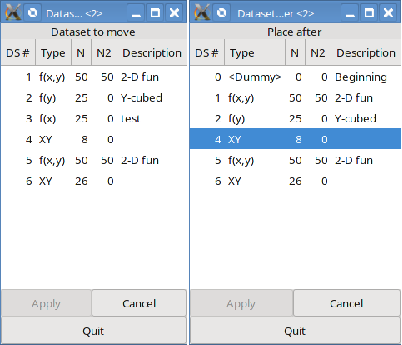
\includegraphics[width=0.5\textwidth]{Sort}
    \caption{Dataset sorting selectors. Left: initial selection, Right:
      target selection.}
    \label{fig:sort}
  \end{figure}
  Multiple datasets may be moved in one invocation, but the ``Do it''
  button is disabled when there is an incomplete move (i.e.\ after a
  dataset has been selected but not relocated).

\item [Merge:]Join two datasets together. The merge option generates a
  pop-up menu with two selector menus each with a list of all the
  observational datasets in the file.


  To use it, first select the dataset to be extended from the left hand
  panel. This will enable all the compatible datasets in the right-hand
  panel, select the one you want to add. 

\begin{quote}
  \textsf{\textbf{HINT:}} \textsf{To make a dataset consisting of two
    existing datasets, while retaining both the originals: create a
    {}``New'' dataset and then merge each of the existing datasets into
    that dataset.}
\end{quote}
\end{description}
To select which Y-axis to use (when a secondary Y-axis is enabled),
there is a pulldown menu adjacent to the input options.

\subsection{Display style}


\subsubsection{1-Dimensional data}

Most of the style options for plot traces that IDL would provide are
available. These are set with the various entry windows and pull down
menus below the plot window. Note that these options are identical for
functions and for observational data.

\begin{description}
\item [Symbol:]The symbol to use for plotting the points. The pull down
  menu has images of the symbols, and displays the current one on the
  undisturbed button. The default is a continuous plot. There are now
  several extra symbols beyond the default IDL symbol set.
\item [Join:]Set the type of line to join the points. This can be
  straight lines joining the points, a histogram type line or no line
  at all.  Note that no symbol and no line is allowed and will result
  in the trace becoming invisible.
\item [Size:]The size to use for the plotting symbols as a multiple of
  the default size. This is ignored for continuous or histogram plots.
  Any floating point value is accepted. 
% The symbol size also determines
%   the length of the caps on error bars.
\item [Line~style:]Line style to use for continuous plots, ignored for
  discrete symbols. The pull down menu shows the available
  styles. Error bars are always drawn with solid lines.
\item [Line~thickness:]The width of the line in terms of the basic line
  width. Enter any real value ($>0. \& \leq100.$) to set the width. This is used
  both for continuous plots and for discrete symbols. Note that at
  least on the printers I use, there is very little visible difference
  between a thickness of 1 and of 2.
\item [Colour:]The colour is set via a pulldown. Most colours have
  names, but some for which I couldn't think of a description are given
  as an RGB triple. There is a difference between \texttt{omit} and
  \texttt{white}: in the first case, the trace is simply not drawn at
  all; in the second, it is drawn in the background colour which will
  overwrite earlier traces and also take time.
\item [Coordinates:]The pull down allows you to select one of three
  coordinate systems:

  \begin{description}
  \item [Rectangular:]The usual X-Y plots.
  \item [Polar~(rad):]Data are $\mathrm{r}$ and $\theta$ values with
    the angles being given in radians.
  \item [Polar~($^{\circ}$):]As above but the angles are given in
    degrees.
  \end{description}
  When the system is changed, the interpretation of the values changes,
  the values themselves are unaltered.

\item [Extra~options:]The \texttt{Extra} button generates a pulldown
  that allows the toggling of some special options:

  \begin{description}
  \item [X-axis~sorting:]For continuous plots, it is possible to
    request that GRAFFER sort the x-axis points into ascending order
    before plotting them. Obviously it has no visible effect if
    discrete symbols are in use.
  \item [Clipping:]Normally plplot clips plots at the axis box, however
    there are times when it is desirable to let a plot go over the
    box. To do this switch the \texttt{Clip to box} option to
    \texttt{Off}.
  \item [Mouse~editing:]For observational data it is usually possible
    to enter, modify and delete points using the mouse, however this
    may not be desirable so is disabled by default; you can use the
    \texttt{Mouse editing} option to allow the current dataset to be
    changed with the mouse.
  \end{description}
\end{description}

\subsubsection{2-Dimensional data}

For 2-D data there are also many options as to how to plot the data
than there are for line plots. The display options are now divided into
two notebook tabs which allow you to toggle between contours and an
{}``image'' format (a third tab allows you to hide the dataset).  In
each case, the menu below the choice allows you to set the detailed
options.
\begin{figure}[htbp]
  \centering
  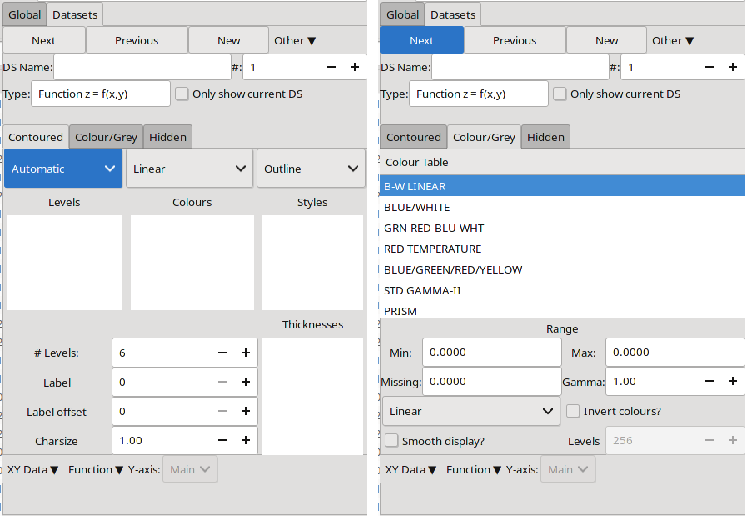
\includegraphics[width=0.8\textwidth]{Main-2}
  \caption{The datasets panel for 2-D datasets with (left) contouring
    options and (right) colour/greyscale options shown.}
  \label{contour}
\end{figure}
\begin{description}
\item [Contoured~display:]The contouring menu
  (\textsc{\autoref{contour})} allows you to specify all the options
  that can be used in a contour plot.

  \begin{description}
  \item [Levels:]The levels can be either explicit, in which case the
    \texttt{levels} entry box is enabled as in
    (\textsc{\autoref{contour})} and levels can be entered one per
    line. The sorting of the levels into increasing order as required
    by the CONTOUR procedure is handled by GRAFFER.


    To use a given number of equi-spaced levels, use the pulldown in
    the top left to select \texttt{Implicit levels}, this will disable
    the levels box and enable the \texttt{\# Levels} box in which you
    can enter how many contour levels you want. This doesn't use IDL's
    internal level setting routines as they do not allow all of the
    other options, so it is done by GRAFFER\footnote{For real
      enthusiasts, the levels are determined as 
      \texttt{levels = rg {*} (findgen(nl)+.5)/nl + mn} where
      \texttt{rg} is the range of the data (ignoring infinities \&
      NaNs), \texttt{mn} is the smallest value in the data and
      \texttt{nl} is the number of levels.}.

  \item [Colours:]Specify the colours of the colour lines (or fill if
    requested).  Unlike the colour settings for line plots, these are
    given by index, the interpretation of the indices is given in%
    \begin{table}[!ht]

      \caption{\textit{\label{col_index}The GRAFFER colour indices.}}

      \begin{center}
        \begin{tabular}{|c|rrr|l|}
          \hline 
          Index&      Red&      Green&      Blue&      Name\\
          \hline 
          0&      255&      255&      255&      White (BG)\\
          1&      0&      0&      0&      Black (default)\\
          2&      255&      0&      0&      Red\\
          3&      0&      255&      0&      Green\\
          4&      0&      0&      255&      Blue\\
          5&      0&      255&      255&      Cyan\\
          6&      255&      0&      255&      Magenta\\
          7&      255&      255&      0&      Yellow\\
          8&      255&      127&      0&      Orange\\
          9&      127&      255&      0&      \#7f ff 00\\
          10&      0&      255&      127&     \#00 ff 7f \\
          11&      0&      127&      255&    \#00 7f ff \\
          12&      127&      0&      255&     \#7f 00 ff \\
          13&      255&      0&      127&      Mauve\\
          14&      85&      85&      85&      Dark Grey\\
          15&      170&      170&      170&      Light Grey\\
          16 & 170 & 0 & 0 & Dark Red\\
          17 & 255 & 85 & 85 & Light Red\\
          18 & 0 & 170 & 0 & Dark Green\\
          19 & 85 & 255 & 85 & Light Green\\
          20 & 0 & 0 & 170 & Dark Blue\\
          21 & 85 & 85 & 255 & Light Blue\\
          22 & 0 & 170 & 170 & Dark Cyan\\
          23 & 85 & 255 & 255 & Light Cyan\\
          24 & 170 & 0 & 170 & Dark Magenta\\
          25 & 255 & 85 & 255 & Light Magenta\\
          26 & 170 & 170 & 0 & Dark Yellow (brown)\\
          27 & 255 & 255 & 85 & Light Yellow\\
          \hline
        \end{tabular}
      \end{center}
    \end{table}
    \textsc{\autoref{col_index}}. If the number of colour indices given
    is less than the number of levels plotted, then the indices are
    recycled.
  \item [Thickness:]Specify line thicknesses for the contours.
  \item [Styles:]Specify the linestyles for the contour lines. These
    are based on the standard IDL linestyles, described in the PLOT keywords
    documentation.
  \item [Filled/Outline:]This pulldown allows you to specify filled
    contours.  With a suitable selection of colours this can be a very
    effective way of displaying data but for large datasets it is slow.

  \item [Labelling:] GRAFFER allows you to label every
    $n^{\mathrm{th}}$ contour. Specifying 0 means don't label any
    contours.
  \item[Charsize] The character size to use for contour labels
    (relative to the default).
  \end{description}

\item [Colour/Greyscale~display:]Also referred to as {}``Image''
  display.  To do this, the dataset is warped to fit the data
  coordinate system and the resulting image is displayed. While this
  can make a nice display it has two serious drawbacks:

  \begin{enumerate}
  \item The smooth display method is slow, seriously slow on a small machine.
  \item It completely obscures all earlier datasets.
  \end{enumerate}
  When this option is selected, then the {}``image'' options menu
  (\textsc{\autoref{contour}}) is displayed. The options are rather
  simpler than those for a contour plot:

  \begin{description}
  \item [Colour~table:]Select any of the available colour tables; when
    the menu appears, the current table will be shown highlighted.
  \item [Range:]The range of values to map from {}``black'' to
    {}``white''.  If these are both zero, then the minimum and maximum
    of the data are used.
  \item [Gamma:]The power-law to use in mapping colour indices to the
    data values (see the LOADCT \& XLOADCT documentation). In essence a
    value of $\Gamma$ less than 1 puts most of the colours at the lower
    end of the data range.
   \item[Log mapping?] Select whether to map the colours
    logarithmically. Note that this will only work with a
    positive-definite dataset or explicit range with both limits
    positive.
  \item[Invert colours?] Select whether to map the colours with the
    high values at the dark end of the table.
  \item[Smooth Display?] When this is set, GRAFFER uses plplot's
    \texttt{plshades} routine to display the image, when unset,
    \texttt{plimage} is used.The first is prettier as is doesn't have
    hard pixel edges but is much slower especially for large datasets
    with a lot of structure.
  \end{description}
\item[Hidden:] If this is selected, then the dataset is not
  displayed. There are no options.
\end{description}

\section{File-wide settings}

While the options discussed in the preceding pages have applied only to
specific datasets, others apply to the whole file. These options are
set from the \textsf{general} tab to the left of the main plotting
window.


\subsection{General settings}


\subsubsection{Plot annotation}

The plot titles and subtitles can be entered in the appropriate boxes
at the top of the general settings menus. The only subtlety to be aware
of is the plotting string escape sequences. To prevent excessive error
messages, the plot is not updated if any annotation string ends with a
single exclamation mark.


\subsubsection{General style}

The character size and line width settings allow you to specify:

\begin{enumerate}
\item The character size for all annotations (the relation between the
  sizes of the title, subtitle and axis labels is defined by plplot and
  GRAFFER does not try to change these (it can be done but the defaults
  are pretty good and it would be a horrible job to fit in all the
  extra setting boxes).
\item The line thickness used for the axes (again in principle you
  could set the axis line widths separately but it would usually be
  ugly and there isn't room for the controls).
\end{enumerate}

\subsubsection{Geometry}

For most purposes the default plotting region is perfectly
adequate. However there are occasions when you need more precise
control of the shape of the plot and the size of its margins. If and
when you do need this capability, the \texttt{Corners...} button
generates a pop-up menu to set these options.

There are two ways of specifying the plot geometry:

\begin{description}
\item [By~region:]This sets the corners of the axis box in normalized
  coordinates. To use this select the \texttt{Corners} option on the
  pulldown at the top of the menu and enter the x \& y coordinates of
  the lower left and upper right corners in the boxes. The \texttt{Do
    it} button will not be enabled until the values are legal, so you
  can't crash it!
\item [By~aspect~ratio:]This 
  defines the corners such that the aspect ratio of the plot is
  preserved even if it is sent to different shaped pages. To use this
  select the \texttt{Aspect ratio} option of the top pulldown and enter
  the aspect ratio (defined as the length of the Y axis divided by the
  length of the X axis) and a margin size. The margin size is expressed
  as a fraction of the page size, and this is interpreted such that the
  smaller margin will be that large and the other will be as large as
  needed to achieve the required aspect ratio.
\item[Isotropic:] Enabling this check box, forces the scales on both
  axes to be identical. The actual sizing of the plot then uses plplot's
  defaults. This option only applicable to the primary Y axis.
\end{description}
To restore the default margin settings, invoke the pop-up and click on
the \texttt{Defaults} button


\subsubsection{Key or legend}

Plots with several traces on them are often useful, but without some
explanation no-one other than the person who drew the plot will know
what the traces are. For this reason GRAFFER provides a mechanism for
adding a key to the plot.
\begin{figure}[htbp]
  \centering
  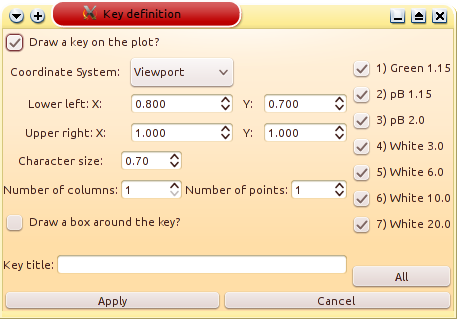
\includegraphics[width=0.8\textwidth]{key}
  \caption{The key (or legend) definition menu of GRAFFER.}
  \label{key menu}
\end{figure}

Pressing the \texttt{Add key} button creates the key definition pop-up
(\textsc{\autoref{key menu}}). The first time you invoke this (for any
given GRAFFER file), the menu will be disabled apart from the
\texttt{Draw a key on the plot?} pulldown at the top; only when that
pulldown is set to \texttt{Yes} does the rest of the menu become
accessible. The menu can conceptually be split into two halves. The
left-hand side specifies the properties of the key while the right
specifies which datasets are to be included.

The location of the menu is specified by giving the coordinates of the
lower left and upper right corners in one of three coordinate
systems\label{coordsys}:

\begin{description}
\item [Data:]The coordinates are given in the same coordinate system as
  the data being plotted. This system has the property that if you
  change the axis limits, the key will remain fixed relative to the
  traces.  If you change the plot geometry (see above), the whole plot
  will change in a self-similar way. It is often difficult to figure
  out just what the box will look like especially in logarithmic
  plots. Data coordinates always use the primary Y-axis.
\item [Normalized:]The coordinates are given in coordinates which run
  from $(0,0)$ in the lower left corner of the page to $(1,1)$ in the
  upper right corner of the page. This means that the key box is fixed
  relative to the page and will move relative to the axes if the plot
  boundaries are moved and relative to the traces if the plot limits
  are changed. Strictly these GRAFFER uses ``region'' coordinates so
  that the location is correct when hard-copy aspect ratio is selected.
\item [Frame:]This system (which is implemented by GRAFFER not by IDL)
  is similar to the Normalized system, but measured relative to the
  corners of the axis box. This means that the plot behaves in a
  self-similar way when you change the boundaries, and the key remains
  fixed relative to the axes when you change the limits. With a
  suitable boundary setting you can put the key outside the axis box by
  using coordinates outside the range 0 to 1. \textbf{This is the
    default system.}
\end{description}

If the default character size is not suitable, then it can be adjusted
by entering a scale factor in the ``Character size'' box, this is a
factor relative to the default (which depends on the size of the axes
and also the global charater size setting).

If you have a secondary Y-axis, then checking the ``Show Y side'' box
adds \texttt{(l)} or \texttt{(r)} after the description to indicate
which axis is applicable to that dataset.

You can arrange the items in the key in any number of columns (although
in practice more than 2 tends not to work very well), just enter the
number of columns you want in the box.

There are two possible formats for the line sample each of which has
advantages and disadvantages:

\begin{description}
\item [1~point:]Plot a short horizontal line segment (if there are
  lines) with a single symbol (if any) in the centre. This is the more
  compact layout and usually looks better, but it cannot distinguish
  normal lines from histogram formats.
\item [2~point:]Plot a sloping line segment with a symbol at each end.
  This needs a little more room and can look untidy but does
  distinguish sloping-line traces from histograms. For historical
  reasons this is the default.
\end{description}
The format is determined by the \texttt{1 or 2 points}
pulldown. Another pulldown determines if a box is to be drawn round the
key.

If a title is entered in the \texttt{title} box, then this is written
above the key, spanning all columns for a multi-column key.

The right-hand side of the menu is a selector menu to determine which
datasets will be listed in the key, only the 1-D datasets (observations
and functions) are listed. In addition to the buttons for the
individual datasets, there is an \texttt{All} button which selects all
the datasets (you can then deselect the ones you don't want).

Unfortunately it is not possible to provide a dynamic update to the key
on the plot, so to see what it looks like you need to click on
\texttt{Do it} and then try again if it doesn't work. Note that
datasets with a colour of \texttt{Omit} are not included even if they
are selected (but they will appear as soon as the colour is changed).


\subsection{Axis settings}

The settings for the axes are identical and so I will only describe a
generic axis setting. Almost all of the standard axis styles that are
available in IDL are available along with a number of extensions.

\begin{description}
\item[Enable~secondary~Y-axis?] (Y-only) This check box is used to
  enable/disable the secondary Y-axis. When it is disabled, then the
  contents of the ``secondary'' tab are desensitised, as is the Y-axis
  selector on the dataset menu.
\item[Main/Secondary] (Y-only) Tabs to select whether to adjust the
  primary or secondary axis.
\item [Label:]The axis label can be entered via the label box. Remember
  that the exclamation mark is an escape character.
\item [Style:]This pulldown covers a multitude of sins, including but
  not limited to the IDL {[}XY{]}STYLE key settings. Each option
  generates a further pulldown of sub-options. Where appropriate, the
  selected sub-option is indicated by an asterisk.

  \begin{description}
  \item [Logarithmic/Linear:] Select whether to plot a linear of
    logarithmic axis. If the axis range is not positive definite, then
    this option is disabled.
  \item [Exact~range:] By default GRAFFER rounds the
    axis limits to some {}``nice'' range which covers the requested
    axis range. If however you really want an exact range, this can be
    forced by setting the exact range option to \texttt{On}.
  \item [Extended~range:] If this is switched on the the axis is
    extended by a small amount (5\%) from the requested limits. This
    operates \textit{after} any rounding.
  \item [Suppress~axes:] Normally GRAFFER draws an axis on each side of
    the plot (thus producing a full box). Both axes can be turned off
    by setting this option on.
  \item [Suppress~box~axis:]Turning this option on just
    suppresses the axis to the right or above the plot. If the draw
    axes option is turned off then it has no effect. This option is
    disabled for the Y-axes when a secondary Y-axis is enabled.
  \item [Minor~ticks:] GRAFFER does not have room to provide full
    support for arbitrary control of the number of minor tick marks. If
    this option is set to \texttt{On} (the default) GRAFFER determines the
    number of minor ticks to add, when it is \texttt{Off} then minor
    ticks are suppressed. For finer control, use the settings in the
    ``Advanced'' menu.
  \item[Label along Axis:] Only available for the Y axes. Set this to
    write the axis labels along the axis rather than horizontally,
    useful if they run into the axis title or off the page.
  \item[Suppress Annotations:] This option allows the suppression of
    the normal labelling of the axis.
  \item [Time~labelling:]Normally only used on the X-axis, but you
    might want it on Y and it's easier to provide the option than to
    omit it.  This option provides some support for
    labelling an axis with times.  When it is switched \texttt{On} then
    a pop-up appears to ask you the units in which the time is given,
    what is the largest unit you wish to put on the plot (e.g. if the
    values are in hours, you might want to label the axis in days and
    hours) and the label to give to the zero point (this is given in
    the largest unit displayed---the idea behind this is to allow a
    date to be added to an axis whose times are in hours of a given
    day). The largest supported unit is days.

\begin{quote}
  \textsf{\textbf{Example:}} \textsf{Suppose you have a time series
    lasting a couple of days starting on 24 February 1997 and the times
    are given in hours from 00:00 UT on 24 Feb. The you should set the
    time unit to} \texttt{hours}\textsf{, the {}``display to'' unit to}
  \texttt{days} \textsf{and the zero value to 24. You should them label
    the axis (say)} \texttt{February 1997}\textsf{.}
\end{quote}
\item [Origin~Axis:]If this option is turned on, then add an
  axis going through the origin of the other axis (if that is on the
  plot). For the X-axis, if a secondary Y axis is plotted, the X-axis
  will be placed at the zero of the primary Y axis. For the
  Y-axis, annotations are suppressed if an origin axis is selected for
  both Y-axes.
\item [Grid:]If this is set to a line style, then extend the major tick
  marks to form a grid and draw them with the given style.
\item [Autoscale:]This isn't really a style option as such, but a means
  of updating the axis limits (see below) to accommodate the
  data. There are two possible ways to do this:

  \begin{description}
  \item [Extend:]This will increase the upper limit, or decrease the
    lower limit so as to include all the datasets within the range.
  \item [Extend~or~shrink:]This will also raise the lower limit or
    lower the upper limit to remove blank space.
  \end{description}
  In either case for Y-axes, if a secondary axis is enabled, then only
  those datasets plotted against that Y-axis are scanned.
\item[Advanced ...] This option allows you to specify some more
  advanced options for axis labelling, via a separate menu
  (Figure~\ref{fig:adv-axis-menu}). Current
  settings available are:
  \begin{figure}
    \centering
    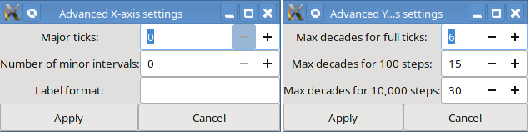
\includegraphics[width=0.8\textwidth]{Axis-adv}
    \caption{The menu for setting advanced axis options. Left: linear
      axes, Right: log axes.}
    \label{fig:adv-axis-menu}
  \end{figure}
  \begin{itemize}
  \item Spacing of the major ticks (this differs from the IDL version
    which specified a number of major ticks).
  \item The number of minor tick intervals, this overrides the simple
    on/off setting of the minor ticks option above.
  \item The format for the tick annotations, this should be a valid
    Fortran format specifier. Note that in order for plplot's default
    formatting to work properly, here the escape character is plplot's
    defualt of \texttt{\#}.
  \end{itemize}
  Setting these to zero or an empty string will use GRAFFER's defaults.
\end{description}
\item [Limits:]The Min and Max boxes allow you to set the axis
  range. If the range requested is invalid, then the plot will not be
  updated until a valid range is entered (this prevents GRAFFER
  crashing while you are editing the numbers). To scale the axis to the
  data, use the Autoscale option of the Style pulldown.
\end{description}

\section{Text}
\label{sec:text}

In addition to the standard plot labels and the key options, GRAFFER
also has facilities to add text at arbitrary locations on the plot.  To
use this facility, you must switch GRAFFER to text mode which makes it
interpret mouse button clicks in the plot window as text operations
instead of dataset operations. The mode button is a pulldown just below
the global and dataset tabs.  When you are in text mode, the cross
hairs that follow the cursor change from continuous to dashed and
extend over the whole window rather than just the axis box.

The button assignments are essentially the same as for the mouse
dataset editing operations, i.e. the LEFT button adds a new text item
at the location of the pointer, the CENTRE button initiates the text
editor on the existing string whose anchor point is closest to the
pointer and the RIGHT button deletes the string whose anchor is nearest
the pointer. Both the edit and delete operations have a maximum
distance of 5 pixels. For the edit operation, if a clcik is more that 5
pixels from any anchor point, then a chooser menu appears to allow you
to select any annotation.

\begin{figure}[htbp]
  \centering
  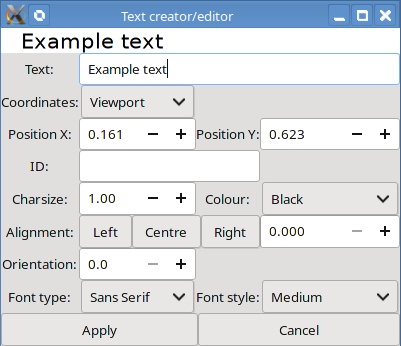
\includegraphics[width=0.8\textwidth]{text}
  \caption{The text input/editing menu of GRAFFER.}
  \label{text panel}
\end{figure}
Insertion of new text and editing of existing text are both
accomplished via the same text input pop-up (\textsc{\autoref{text
    panel}}). There are many user-settable fields in the menu:

\begin{description}
\item [The~text~string:]This is a text entry widget into which
  you can type the text string to be displayed. Any of the IDL graphics
  controls ( !<\textit{char}> commands) may be used as these text
  strings are displayed in vector fonts (unless of course you have
  specifically requested hardware font). As you type the text into the
  box, it will be reflected in the graphics window above in the size,
  font etc. in which it will appear on the plot. If no text string is
  given it will be displayed as \texttt{<NULL>}, this will not be
  printed on a hard copy, nor is it displayed while editing the
  text. Also, text items after the current one may not appear while
  editing is in progress.
\item [Coordinate~system:]A pull down to select Data, Normalized or
  Frame coordinates as the system in which the text is anchored. The
  default is data, but if you wish the text to remain in the same place
  on the page when you change the axis range, then use normalized, if
  you want the text fixed relative to the axes use Frame. For more
  details of the systems see p~\pageref{coordsys}.
\item[Y-axis:] If a secondary Y-axis is available, then this allows you
  to select which one to use for Data coordinates. This selector is not
  created when there is no secondary Y-axis, and is disabled when the
  coordinate system is not Data. By default, the coordinate system of
  the current dataset is selected.
\item [Position:]Set or adjust the position of the anchor point, both X
  and Y are floating-point numbers and are given in the currently
  selected coordinate system.
\item[ID:] An identification string. Mainly for use to select an
  annotation for the gdl/idl programmatic tools.
\item [Character~Size:]Enter a floating-point value to give the
  character size in terms of the default value. When hard copies are
  made, the size is adjusted to give the same number of characters
  across the page as were on the screen.
\item [Colour:]The colour of the text, the pulldown has the same
  colours as for plot traces, except that there is no option to omit
  the text entirely. In the figure the ``alternate'' colour pixmap
  selector is enabled.
\item [Justification:]A pull down which allows you to set Left, Centre,
  Right or otherwise-justified text. 
\item [Orientation:]Set the orientation of the text. This is measured
  in degrees anti-clockwise from the normal position of parallel to the
  X-axis and going left to right.
\item [Font:] A pair of pull downs to select the font. The first
  selects the font, and the second the shape.
\end{description}
In order to reduce the refresh time as you are typing the text string,
the plot is not updated after every character you type, instead the
string is displayed in a small window at the top of the text entry menu
(the only characteristic which is ignored is the orientation).  The
\texttt{Apply} and \texttt{Cancel} buttons have their usual meanings.

Remember that when you are in text mode you cannot then use the mouse
to edit datasets, however all other dataset operations remain valid.


\section{Control}

In this section I shall describe the various {}``control'' operations
that allow GRAFFER to deal with the outside world and thus be useful.
All of the operations are controlled from the buttons on the top-left
of the GRAFFER control panel.


\subsection{Hard Copy}

GRAFFER supports the generation of PostScript and PDF hard copy files
(and also export to SVG) with a wide range of options. When requesting
hard copy you can retain the current options (or the defaults if none
have been set) by selecting the relevant option of the
pulldown. If you select the \texttt{Options} menu item, then the hard copy
setup menu will be produced (\textsc{\autoref{hardcopy menu}}).

 \begin{figure}[htbp]
   \centering
   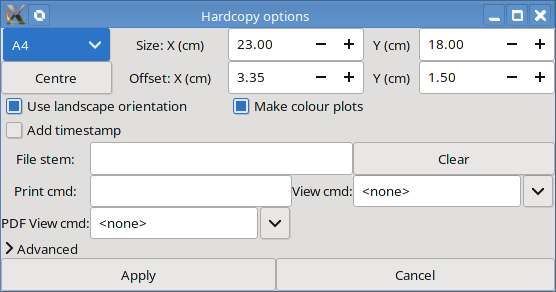
\includegraphics[width=0.6\textwidth]{hardcopy}
   \caption{The GRAFFER hard copy set up menu.}
   \label{hardcopy menu}
 \end{figure}
 The size and placement of the plot can be controlled by the buttons
 and entry boxes in the first few lines of the menu:

 \begin{description}
 \item [Paper~size:]Allows you to toggle between the European A4
   ($210\times297\mathrm{mm}$) (default) and American Letter
   ($8.5\times11^{\prime\prime}$) paper sizes. Plplot doesn't put paper
   size commands into its PostScript output\footnote{This is a good
     thing as if a file with embedded paper size commands is sent to a
     printer with different sized paper it will typically hang the
     queue until someone intervenes.} so this is just used in GRAFFER's
   internal accounting to figure out margins etc.
 \item [Centre~on~page:]Adjust the offsets so that the current page
   size is centred on the paper; note this is not a retained
   characteristic so you have to re-apply this any time you change the
   page dimensions. (Disabled for EPS).
 \item [X~\&~Y~sizes:]Set the X \& Y dimensions of the page. The X \& Y
   directions correspond to the directions of the axes on your plot.
   Note that there is nothing to stop you making a portrait orientation
   file with the X dimension larger than the Y, in fact this is the
   recommended way of making landscape encapsulated files.
 \item [X~\&~Y~offsets:]Set the distance between the lower left corner
   of your plot page and the lower left corner of the page. Again this
   refers to the corners as seen when you are looking at the plot in
   the usual way people look at plots, GRAFFER handles the axis
   interchanging needed (but it will get it wrong if you don't tell it
   the right paper size!).
 \end{description}

 The other {}``formatting'' options are:

 \begin{description}
 \item[Use landscape orientation] If this is selected, then the page is
   oriented with the longer axis as X. In plplot this is not really
   very important.
 \item[Make colour plots] This selects (theoretically) colour or
   monchrome plot generation, however the cairo driers do not appear to
   honour the relevant plplot call.
 \item [Add~timestamp:]If this is selected, then add a string with the
   date of generation and the username of the generator to the plot.
 \end{description}

The final few items set the output file options
\begin{description}
\item[File stem] The default output file is derived from the GRAFFER
  file name by replacing the suffix with \texttt{.ps}, \texttt{.eps} or
  \texttt{.pdf} according to the selected output. This can be changed
  via the output file entry box.
\item[Clear] Clear the file name stem, will then be generated from the
  GRAFFER file name.
\item[Print cmd, View cmd] 
 For ``normal'' PostScript files, GRAFFER can automatically spool
 the file to the printer, this can.  A view for encapsulated postscript
 can be chosen in the ``View cmd'' box (this is an editable combobox
 that offers the known suitable viewers as choices). There is
 (currently) no automatic disposal of pdf files.
\end{description}

This menu also allows you to select specific \texttt{plplot} device
drivers for the various output formats if you so wish.

The \texttt{Cancel} and \texttt{Apply} buttons have their usual
meanings.


\subsection{Saving and dumping}

One of the key features of GRAFFER is that you can save you plot to a
file and then come back to it later. The various saving options are
under the \texttt{File} menu, there is also a sub-menu to allow you to
make screen dumps.

There are three save options which allow you to save to the current
file in the current format or to save to a specified file in either
binary or ASCII format.

Normally binary files are preferable as they are smaller and quicker to
read and there is no risk of losing precision in floating point
numbers. However if you want to transfer the file to a different
platform then you should use ASCII as the representations of the
numbers may differ\footnote{Unfortunately I was not able to devise an
  automatic means of distinguishing binary, ASCII and non-GRAFFER files
  if I used XDR for the binary form.  Abandoning ASCII would have meant
  that version 1 could not be read into version 2. For machines with
  IEEE floating point formats (most machines nowadays) binary files can
  be read irrespective of endianness by the simple expedient of
  checking the version number and swapping bytes if the raw version
  number is greater then 255.}.

If you request a save to a new name, a pop-up will appear to allow you
to edit the new filename. If you try to save over an existing filename,
a warning will be given and you will have the option of overwriting or
trying another name.

The screen dump allows you to dump the GRAFFER plot window to a PNG,
TIFF or JPEG file, the name will be the current filename with an
appropriate extension.


\subsection{Opening a new file}

When you start GRAFFER you either give it a file name as an argument,
or you use a picker to select or specify a file name. If you wish to
work on another file, you don't have to leave GRAFFER and restart as
the \texttt{Open} options allow you to change file without exiting.

\begin{description}
\item [Open~restore:]This will start up the same picker that is used
  when you enter GRAFFER without an argument. The only difference is
  that you can't select a non-existent file.
\item [Open~new:]This starts a pop-up that allows you to enter the name
  and directory of a new file. If you specify a file that already
  exists, you will be given the opportunity to try something else
  before it is overwritten, however the existing file will \textbf{not}
  be opened.
\end{description}

\subsection{Options...}
\label{sec:options}

\begin{figure}
  \centering
  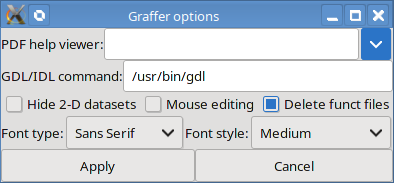
\includegraphics[width=0.5\textwidth]{options}
  \caption{The options menu dialogue.}
  \label{fig:options}
\end{figure}
The ``Options...'' item in the \texttt{Settings} control menu allows
you to set a number of options, via a pop-up dialogue
(\textsc{\autoref{fig:options}}).

\begin{description}
\item[PDF Viewer] Select the program to use to view the PDF help files.
\item[Hide 2-D data] Toggles the display of 2-D datasets (allows the
  display of contour and image data to be suppressed on slow machines).
\item[Mouse editing] Controls whether mouse editing is allow on
  new datasets.
\item[Delete funct files] This controls whether GRAFFER deletes the
  program and data files generated in evaluating functions.

\item[Font type, Font style] These pulldown menus allow you to control
  the font used for the labels and annotations on the plot.
\end{description}

The \texttt{Settings} submenu also has an option to allow you to add
extra colour tables for ``image'' display. By default files called
\texttt{*.table} are searched. The details of the format are described
at the end of the File formats manual.

\subsection{Exit and Help}

The \texttt{Exit} item in the \texttt{File} menu exits from GRAFFER to
the \texttt{IDL>} prompt, it does not exit from IDL. If the file is
changed, you will be given the opportunity to save it or abort the
exit.

The \texttt{Help} button launches a browser to look at a PDF version of
this manual. In addition in the main menu, and many others tooltips are
provided to explain the function of the setting widgets when the cursor
is held over that widget.

\section{Accelerator Keys}
\label{sec:accel}

In version 3.04, accelerator keys were added to the main menu.

The following accelerators are defined:
\begin{description}
\item[Ctrl-Q] Quit.
\item[Ctrl-S] Save.
\item[Ctrl-Shift-S] Save binary as.
\item[Ctrl-P] Hard copy -- quick.
\item[Ctrl-Shift-P] Hard Copy -- set up.
\item[Ctrl-N] Open new file.
\item[Ctrl-O] Open existing file.
\item[Ctrl-H] Show user manual.
\item[f, F11] Toggle full screen -- make the GRAFFER window into a full
  screen view, can also be exited with ``Escape'', only applicable when
  the cursor is in the drawing area. Fortran version only.
\end{description}

\part{GDL/IDL procedures}
\label{part:gdl}

These procedures which allow the user to create and update GRAFFER
files from within \texttt{gdl} or \texttt{idl} are extracted from the
original IDL version. All should work in \texttt{gdl} as well.

\section{GRAFF\_ADD (interface user programs to GRAFFER)}
\label{sec:graff_add}

This is all very well but suppose you have a procedure that generates
radial spokes on a series of images and you want to use GRAFFER to make
up a plot of these radial spokes it's going to be rather tedious to
specify all the slices to the top-level variable reader, or write them
to a series of files and then load each file. To automate this and
indeed to allow the use of variables which are never passed back to the
top-level to be used there is a procedure GRAFF\_ADD. GRAFF\_ADD adds
datasets to a GRAFFER file, if need be the file is created, it cannot
delete datasets or replace existing datasets, also some of the more
complex options cannot be set up by GRAFF\_ADD.

N.B. For this an all other programatic \texttt{graffer} tools, you can
check for possible extra keywords by using the command:
\begin{verbatim}
doc_library, 'graff_add'
\end{verbatim}
or whichever routine you want to check at the \texttt{IDL>} prompt.

\subsection{Interface}

\begin{verbatim}
 graff_add, file, [[[z], x,] y, errors=errors, x_func=x_func, $
         y_func=y_func, errtype=errtype, z_func=z_func, $
         polar=polar, rescale=rescale, /display, join=join, $
         style=style, psym=psym, symsize=symsize, colour=colour, $
         thick=thick, neval=neval, description=description, $
         frange=frange, /ascii, /noclip, $
         mouse=mouse,z_format=z_format, z_nlevels = z_nlevels, $
         z_levels = $ 
         z_levels, z_colours = z_colours, z_style = z_style, $
         z_thick = z_thick, z_range = z_range, z_label = $
         z_label, z_pxsize = z_pxsize, z_invert = z_invert, $
         z_fill = z_fill, z_log=z_log, z_ctable = z_ctable, $
         xy_file = xy_file, z_file = $
         z_file, func_file = func_file, y_axis=y_axis]
\end{verbatim}

\subsection{Arguments}

\begin{description}
\item[\texttt{file} \textit{string}] The graffer file to modify.
\item[\texttt{z} \textit{float}] The Z values for a 2-D dataset (If
  only 2 arguments are present, then they are treated as X \& Y)
\item[\texttt{x} \textit{float}] The x values to add.
\item[\texttt{y} \textit{float}] The y values to add.
\end{description}



\subsection{Keywords}

\begin{description}
\item[\texttt{errors} \textit{float}] Array with errors, 1-d or (m,n).
\item[\texttt{errtype} \textit{string}] Specify error types as code see
  \textsc{\autoref{ecodes}}
\item[\texttt{x\_func} \textit{string}] Function specification for x =
  f(y) or x = f(t)
\item[\texttt{y\_func} \textit{string}] Function specification for y =
  f(x) or y = g(t)
\item[\texttt{z\_func} \textit{string}] Function specification for z =
  f(x,y)
\item[\texttt{frange} \textit{float}] The range of x, y or t over which
  to plot a function
\item[\texttt{polar} \textit{int}] If unset or 0 rectangular, 1 = polar
  in radians, 2 = polar in degrees.
\item[\texttt{rescale} \textit{flag}] If set, then reset the scaling of
  the plot with the autoscale routine.
\item[\texttt{display} \textit{flag}] If set, then display the plot on
  the current device.
\item[\texttt{style} \textit{int}] The standard IDL linestyle codes
\item[\texttt{psym} \textit{int}] The GRAFFER symbol code - extended
  IDL symbol codes
\item[\texttt{join} \textit{int}] The style of joining: 0 - none, 1 -
  sloping lines, 2 - histogram
\item[\texttt{symsize} \textit{float}] The size for the symbols
  (relative to standard)
\item[\texttt{colour} \textit{int}] Colour number - standard GRAFFER
  colours
\item[\texttt{thick} \textit{float}] Line thickness.
\item[\texttt{neval} \textit{int}] The number of times to evaluate a
  function. (2-elements for \texttt{z\_func})
\item[\texttt{description} \textit{string}] A description of the data
  set.
\item[\texttt{sort} \textit{flag}] Whether to sort the values on the
  X-axis
\item[\texttt{ascii} \textit{flag}] If set, then save as an ASCII
  GRAFFER file (default is binary)
\item[\texttt{noclip} \textit{flag}] If set, then disable clipping to
  the axis box.
\item[\texttt{mouse} \textit{int}] If explicitly set to zero then
  disable mouse-editing of the dataset.

\item[\texttt{z\_format} \textit{int}] 2-D datasets, select
  displayformat (0=contour, 1=colour image)

\item[\texttt{z\_nlevels} \textit{int}] For 2D datasets, select number
  of automatic contours

\item[\texttt{z\_levels} \textit{float}] For 2D datasets, select levels
  for explicit contours

\item[\texttt{z\_colours} \textit{int}] For 2D datasets, select the
  colours for the contours

\item[\texttt{z\_style} \textit{int}] For 2D datasets, select
  linestyles for contours

\item[\texttt{z\_thick} \textit{float}] For 2D datasets, select line
  thicknesses for contours

\item[\texttt{z\_label} \textit{int}] Specify the interval of contours
  for labelling.

\item[\texttt{z\_fill} \textit{flag}] If set, then fill the contours.

\item[\texttt{z\_range} \textit{int}] For 2-D datasets, specify the
  cutoff range for image displays

\item[\texttt{z\_pxsize} \textit{float}] For 2D datasets, specify the
  pixel size to use in images for PS device.

\item[\texttt{z\_invert} \textit{flag}] For image display, invert the
  colour table if set.

\item[\texttt{z\_log} \textit{flag}] If set, then map the Z values
  logarithmically.
\item[\texttt{z\_ctable} \textit{int}] Select a colour table for 2-D
  display of images.
\item[\texttt{xy\_file} \textit{string}] A file with a graffer dataset
  (x-y plot).
\item[\texttt{z\_file} \textit{string}] A file with a graffer dataset
  (2-D data).
\item[\texttt{func\_file} \textit{string}] A file with a graffer
  function dataset.
\item[\texttt{y\_axis} \textit{int}] Select which Y-axis to scale this
  data to. (Set but ignored if the file does not have a secondary
  Y-axis).
\end{description}



\subsection{Restrictions}

\begin{itemize}
\item The \texttt{func<xyz>} keys and the x,y,z arguments are
  exclusive.
\item The \texttt{GRAFFER} key overrides the \texttt{DISPLAY} key and
  the \texttt{ASCII} key.
\item There is no support for deleting or replacing datasets.
\end{itemize}


\section{GRAFF\_PROPS (set GRAFFER file properties programmatically)}
\label{sec:graff_props}

This procedure is the global counterpart of \texttt{GRAFF\_ADD}, and
allows you to set various options from your program.


\subsection{Interface}
\label{sec:gp_interface}

\begin{verbatim}
graff_props, file, title=title, subtitle=subtitle, $
         charsize=charsize, thick=thick, corners=corners, $
         aspect=aspect, comment=comment, xtitle=xtitle, $
         xrange=xrange, xlog=xlog, xexact=xexact, $
         xextend=xextend, xaxes=xaxes, xbox=xbox, $
         xminor=xminor, xtime=xtime, xorigin=xorigin, $
         xgrid=xgrid, xauto=xauto, $
         ytitle=ytitle, $
         yrange=yrange, ylog=ylog, yexact=yexact, $
         yextend=yextend, yaxes=yaxes, ybox=ybox, $
         yminor=yminor, ytime=ytime, yorigin=yorigin, $
         ygrid=ygrid, yauto=yauto, yr_enable = yr_enable, $
         yrtitle=yrtitle, $
         yrrange=yrrange, yrlog=yrlog, yrexact=yrexact, $
         yrextend=yrextend, yraxes=yraxes, $
         yrminor=yrminor, yrtime=yrtime, yrorigin=yrorigin, $
         yrgrid=yrgrid, yrauto=yrauto, ascii=ascii, h_orient=h_orient, $
         h_colour=h_colour, h_eps=h_eps, h_xsize=h_xsize, $
         h_ysize=h_ysize, h_xmargin=h_xmargin, $
         h_ymargin=h_ymargin, isotropic = isotropic, h_cmyk = $
         h_cmyk, ctable = ctable, h_print = h_print, h_viewer $
         = h_viewer, h_file = h_file, h_psdev = h_psdev, $
         h_epsdev = h_epsdev, h_pdfdev = h_pdfdev, h_pdfdev = $
         h_pdfdev
\end{verbatim}


\subsection{Arguments}
\label{sec:gp_args}
\begin{description}
\item[\texttt{file} \textit{string}] The graffer file to modify.
\end{description}


\subsection{Keywords}
\label{sec:gp_key}

\begin{description}
\item[\texttt{title} \textit{string}] Set the plot title.
\item[\texttt{subtitle} \textit{string}] Set the subtitle for the plot.
\item[\texttt{charsize} \textit{float}] Set the character size to be
  used for axis labelling and plot annotations.
\item[\texttt{thick} \textit{float}] Set the line thickness to be used
  for drawing the axes.
\item[\texttt{corners} \textit{float}] Set the location of the plot in
  normalized coordinates by specifying the locations of the corners
  (4-elemant array [x0,y0, x1,y1])
\item[\texttt{aspect} \textit{float}] Set the location of the plot
  within the normalized coordinate system by aspect ratio and margin
  (2-element array [aspect, margin] N.B. Specifying both ASPECT \&
  CORNERS is an error and the plot location is unchanged.
\item[\texttt{isotropic} \textit{flag}] Set the plot to use isotropic
  coordinates.
\item[\texttt{comment} \textit{string}] Set a descriptive comment for
  the whole file. (String array)
\item[\texttt{{[x|y|yr]}title} \textit{string}] Set the title for the
  specified axis.
\item[\texttt{{[x|y|yr]}range} \textit{double}] Set the range of the
  specified axis (2-element array).
\item[\texttt{{[x|y|yr]}log} \textit{flag}] Set or unset the use of
  logarithmic axes.
\item[\texttt{{[x|y|yr]}exact} \textit{flag}] Set or unset the exact
  range bit of the IDL axis style setting
\item[\texttt{{[x|y|yr]}extend} \textit{flag}] Set or unset the
  extended range bit of the IDL axis style setting
\item[\texttt{{[x|y|yr]}axes} \textit{flag}] Set or unset the axis
  plotting bit of the IDL axis style setting.
\item[\texttt{{[x|y]}box} \textit{flag}] Set or unset the "box-axis"
  bit in the IDL axis style setting. Note this is not applicable to the
  secondary Y-axis, and is ignored for the main Y-axis if a secondary
  axis is specified.
\item[\texttt{{[x|y|yr]}minor} \textit{flag}] If set, then display
  minor ticks on the plot; if explicitly zero, then turn off the minor
  ticks.
\item[\texttt{{[x|y|yr]}time} \textit{flag/struct}] If set to zero,
  then turn off time labelling, otherwise this must be a structure with
  the members described in \textsc{\autoref{tab:time}}.
  \begin{table}[htbp]
    \centering
    \begin{tabular}{|l|l|}
      \hline
      \texttt{unit}&  0 == seconds\\
      & 1 == minutes\\
      & 2 == hours\\
      & 3 == days\\
      &  Gives the unit in which the\\
      & time is expressed in the axis data.\\
      \hline
      \texttt{max\_unit}& gives the largest unit to\\
      &   display on the plot (same code as\\
      &  for unit)\\
      \hline
      \texttt{zero} & gives the value to be used for \\
      &  the zero of the axis (expressed in\\
      & units of  max\_unit\\
      \hline
    \end{tabular}
    \caption{Time axis structure}
    \label{tab:time}
  \end{table}
\item[\texttt{{[x|y|yr]}origin} \textit{flag}] If set, then plot an
  axis at the origin.
\item[\texttt{{[x|y|yr]}grid} \textit{flag}] Make a grid from the major
  ticks, using linestyle n-1 (0 == no grid).
\item[\texttt{{[x|y|yr]}auto} \textit{flag}] If set, then perform an
  autoscale on the specified axis, the corresponding range setting
  takes precedence over this setting.
\item[\texttt{yr\_enable} \textit{flag}] Enable/disable the display of
  a secondary Y-axis.
\item[\texttt{ascii} \textit{flag}] If set, then save as an ASCII
  GRAFFER file (by default a binary graffer file is generated).
\item[\texttt{h\_orient} \textit{int}] Set landscape(0) or portrait (1)
  orientation of the page.
\item[\texttt{h\_colour} \textit{flag}] Set or unset the generation of
  a colour (E)PS file.
\item[\texttt{h\_cmyk} \textit{flag}] Set or unset the use of the CMYK
  model for (E)PS files. Specifying this keyword will force colour
  (E)PS.
\item[\texttt{h\_eps} \textit{flag}] Set or unset the generation of EPS
  file rather than PS (N.B. if h\_eps is set and h\_orient is not
  specified, then h\_orient=1 is implied).
\item[\texttt{h\_[xy]size} \textit{float}] Set the X(Y) dimension of
  the page in cm
\item[\texttt{h\_[xy]margin} \textit{float}] Set the X(Y) offset of the
  page from the lower-left corner of the page.
\item [\texttt{ctable} \textit{int}] Set the default colour table for
  image display.
\item[\texttt{h\_print} \textit{string(s)}] Specify the command to
  print PS output files (can be a scalar or 2-element aray).
\item[\texttt{h\_viewer} \textit{string(s)}] Specify the command to
  view EPS output files (can be a scalar or 2-element aray).
\item[\texttt{h\_file} \textit{string}] Specify the output file for
  hardcopies.
\item[\texttt{h\_psdev}	\textit{string}] Specify the PS device driver (plplot).
\item[\texttt{h\_epsdev} \textit{string}] Specify the EPS device driver (plplot).
\item[\texttt{h\_pdfdev} \textit{string}] Specify the PDF device driver (plplot).
\item[\texttt{h\_svgdev} \textit{string}] Specify the SVG device driver (plplot).

\end{description}



\subsection{Restrictions}
\label{sec:gp_restrict}

\begin{itemize}
\item The ASPECT and CORNERS keys are exclusive (if both are given,
  both are ignored).

\item {[X|Y|YR]}RANGE overrides {[X|Y|YR]}AUTO.

\item The GRAFFER key overrides the DISPLAY key and the ASCII key.

\item As yet the addition/modification of a key (legend) is not
  supported.

\item Not all hardcopy options can be set.

\end{itemize}

\section{GRAFF\_UPDATE}
\label{sec:graff_update}

User-callable interface to update the properties of a dataset.

\subsection{Interface}
\label{sec:upd_interface}


\begin{verbatim}
graff_update, file, idx, name=name, polar = polar, rescale = rescale, $
            style = style, psym = psym, join = $
            join, symsize = symsize, colour = colour, thick = $
            thick, neval = neval, description = description, $
            sort = sort, ascii = ascii, noclip = noclip, $
            mouse = mouse, z_format = z_format, z_nlevels = $
            z_nlevels, z_levels = z_levels, z_colours = z_colours, $
            z_style = z_style, z_thick = z_thick, z_range = $
            z_range, z_label = z_label, z_pxsize = z_pxsize, $
            z_invert = z_invert, z_fill = z_fill, z_log = z_log, $
            z_ctable = z_ctable, y_axis=y_axis, $
            make_current = make_current x_values = x_values, $
            y_values = y_values, z_values = z_values, x_func = $
            x_func, y_func = y_func, z_func = z_func, xy_file = $ $
            xy_file, z_file = z_file, errors = errors, errtype = $
            errtype, neval = neval, frange = frange
\end{verbatim}

\subsection{Arguments:}
\label{sec:gu_args}


\begin{description}
\item[\texttt{file} \textit{string}] The graffer file to modify.
\item[\texttt{idx} \textit{int}] input The dataset index to modify
  (starting at 1).
\end{description}

\subsection{Keywords:}
\label{sec:gu-keywords}

\begin{description}
\item[\texttt{name} \textit{string}] Find the dataset to update by
  searching the descriptor fields to match the name.
\item[\texttt{frange} \textit{float}] The range of x, y or t over which
  to plot a function
\item[\texttt{polar} \textit{int}] If unset or 0 rectangular, 1 = polar
  in radians, 2 = polar in degrees.
\item[\texttt{rescale} \textit{input}] set, then reset the scaling of
  the plot with the autoscale routine.
\item[\texttt{style} \textit{int}] The standard IDL linestyle codes
\item[\texttt{psym} \textit{int}] The GRAFFER symbol code - extended
  IDL symbol codes.
\item[\texttt{join} \textit{int}] The style of joining: 0 - none 1 -
  sloping lines 2 - histogram
\item[\texttt{symsize} \textit{float}] The size for the symbols
  (relative to standard)
\item[\texttt{colour} \textit{int}] Colour number - standard GRAFFER
  colours (which may well not work on current device).
\item[\texttt{thick} \textit{float}] Line thickness.
\item[\texttt{neval} \textit{int}] The number of times to evaluate a
  function. (2-elements for z\_func)
\item[\texttt{description} \textit{str}] A description of the data set.
\item[\texttt{sort} \textit{input}] to sort the values on the X axis.
\item[\texttt{ascii} \textit{input}] set, then save as an ASCII GRAFFER
  file (by default a binary graffer file is generated).
\item[\texttt{noclip} \textit{input}] set, then disable clipping to the
  axis box.
\item[\texttt{mouse} \textit{int}] If explicitly set to zero then
  disable mouse-editing of the dataset.
\item[\texttt{z\_format} \textit{int}] For 2-D datasets, select display
  format (0=contour, 1=colour image)
\item[\texttt{z\_nlevels} \textit{int}] For 2D datasets, select number
  of automatic contours
\item[\texttt{z\_levels} \textit{float}] For 2D datasets, select levels
  for explicit contours
\item[\texttt{z\_colours} \textit{int}] input For 2D datasets, select
  the colours for the contours
\item[\texttt{z\_style} \textit{int}] For 2D datasets, select
  linestyles for contours
\item[\texttt{z\_thick} \textit{float}] For 2D datasets, select line
  thicknesses for contours
\item[\texttt{z\_label} \textit{int}] Specify the interval of contours
  for labelling.
\item[\texttt{/z\_fill}] If set, then fill the contours.
\item[\texttt{z\_range} \textit{int}] For 2-D datasets, specify the
  cutoff range for image displays
\item[\texttt{z\_pxsize} \textit{float}] For 2D datasets, specify the
  pixel size to use in images for PS device.
\item[\texttt{/z\_invert}] For image display, invert the colour table
  if set.
\item[\texttt{/z\_log}] If set, then map the Z values logarithmically.
\item[\texttt{z\_ctable} \textit{int}] Select a colour table for 2-D
  display of images.
\item[\texttt{y\_axis} \textit{int}] Select to which Y-axis the dataset
  will be scaled.
\item[\texttt{/make\_current}] If set, then make the modified dataset
  into the current dataset when the file is next opened.
\item[\texttt{x\_values} \textit{double}] New X values.
\item[\texttt{y\_values} \textit{double}] New Y values.
\item[\texttt{z\_values} \textit{double}] New Z values.
\item[\texttt{x\_func} \textit{string}] New x=f(y), or x=f(t)
\item[\texttt{y\_func} \textit{string}] New y=f(x), or y=f(t).
\item[\texttt{z\_func} \textit{string}] New z=f(x,y).
\item[\texttt{xy\_file} \textit{string}] File for new 1-D data.
\item[\texttt{z\_file} \textit{string}] File for new 2-D data.
\item[\texttt{errors} \textit{double}] New error values.
\item[\texttt{errtype} \textit{string}] Specify error types as code
  (e.g. "XXY" for asymmetrical errors in X and symmetric errors in Y)
\item[\texttt{frange} \texttt{float}] The range of x, y or t over which
  to plot a function
\end{description}

\subsection{Restrictions:}
\label{sec:gu-restr}

Does not allow the type of dataset to be changed.  If neither the index
or the name is given, then the current dataset is modified.  Specifying
both is an error.  If name is given then (1) If there are 2 datasets of
the same name, the first will be modified, (2) if the name is not
found, then the program exits without updating.

\section{GRAFF\_EXPORT}
\label{sec:graff_export}


\begin{verbatim}
graff_export, file, index, name = name, outfile = outfile
\end{verbatim}

\subsection{Arguments}
\label{sec:ge-args}

\begin{description}
\item[\texttt{file} \textit{string}] The graffer file.
\item[\texttt{index} \textit{int}] The index of the dataset to write.
\end{description}

\subsection{Keywords}
\label{sec:ge-keys}

\begin{description}
\item[\texttt{name}	\textit{string}] The descriptor of the dataset to write.
\item[\texttt{outfile}	\textit{string}] The file to which to write the dataset
\end{description}

\subsection{Notes}
\label{sec:ge-notes}

If neither the index or the name is given, then the current dataset is
written.  Specifying both is an error.  If name is given then (1) If
there are 2 datasets of the same name, the first will be written, (2)
if the name is not found, then the program exits without writing.

\section{GRAFF\_ANNOTATE}
\label{sec:graff_annotate}

	Add or modify an annotation to a graffer file.

\subsection{Interface}
\label{sec:ga-inter}

\begin{verbatim}
graff_annotate, file[, value, <keywords>]
\end{verbatim}

\subsection{ Arguments}
\label{sec:ga-args}



\begin{description}
\item[\texttt{file} \textit{string}] The file to modify
\item[\texttt{value} \textit{string}] The text of the
  annotation to modify (This is not generally a good way to identify
  the annotation).
\end{description}

 \subsection{Keywords}
 \label{sec:ga-keys}

 \begin{description}
\item[\texttt{id} \textit{string}] The ID tag of the annotation to modify.
\item[\texttt{index} \textit{int}] The index number (1-based) of the annotation
		to modify
\item[\texttt{/substring}] If set, then VALUE may match an initial substring.
\item[\texttt{/case\_squash}] If set, then VALUE is matched without regard
		to case.
\item[\texttt{text} \textit{string}] New text for the annotation.
\item[\texttt{newid} \textit{string}] A new ID for the annotation.
\item[\texttt{colour} \textit{int}] The colour for the annotation.
\item[\texttt{size} \textit{float}] The font size for the annotation
\item[\texttt{orient} \textit{float}] The orientation of the annotation
		(anticlockwise, degrees)
\item[\texttt{align} \textit{float}] The alignment (0=left, 1=right, 0.5=centre)
\item[\texttt{ffamily} \textit{int}] The font family to use 
\item[\texttt{font} \textit{int}] Set the font shape for the desired font.
\item[\texttt{x} \textit{float}] Set the X-coordinate of the origin
\item[\texttt{y} \textit{float}] Set the Y-coordinate of the origin
\item[\texttt{norm} \textit{int}] Set the coordinate system, 0=data,
		1=normalized, 2 = "frame".
\item[\texttt{axis} \textit{int}] For data coordinates, set which Y axis to use.
\item[\texttt{status} \textit{int}] A named variable, set to 1 on success, 0 on
		failure.
\end{description}

\subsection{ Notes}
\label{sec:ga-notes}

	Specifying more than one identification is an error, if no
	identification is given then a new annotation is created.
	For a new annotation, at least TEXT, X and Y must be given

 \section{GRAFF\_GET\_DATA}
 \label{sec:graff-get-data}

 
	Extract data from a graffer file.

 \subsection{Usage:}
 \label{sec:ggd-usage}

 
\begin{verbatim}
graff_get_data, file[, index, <extraction keys>]
\end{verbatim}

\subsection{ Argument:}
\label{sec:ggd-args}

\begin{description}
\item[\texttt{file} \textit{string}] The file to extract.

\item[\texttt{idx} \textit{int}] The dataset index to extract

\end{description}

\subsection{ Keywords:}
\label{sec:ggd-keys}

\begin{description}
\item[\texttt{name} \textit{string}] Specify the dataset by name.
\item[\texttt{xval} \textit{double}] A variable to contain the X
  values.
\item[\texttt{yval} \textit{double}] A variable to contain the Y
  values.
\item[\texttt{zval} \textit{double}] A variable to contain the Z
  values.
\item[\texttt{xerr} \textit{double}] A variable to contain the X
  errors.
\item[\texttt{yerr} \textit{double}] A variable to contain the Y
  errors.
\end{description}

\section{GRAFF\_CONVERT}
\label{sec:graff_convert}


Convert an older Graffer file to the current format.

\subsection{Usage:}
\label{sec:gr_c_use}
        
\begin{verbatim}
graff_convert, file[, ofile]
\end{verbatim}

\subsection{Arguments:}
\label{sec:gr_c_args}

\begin{description}
\item[\texttt{file} \textit{string}] The file to convert
\item [\texttt{ofile} \textit{string}] The new name for the file, if
  not given, then the old file is overwritten.
\end{description}


\subsection*{Acknowledgements}

Thanks to Norbert Hahn of the University of Darmstadt for suggesting
the need for a more compact format for those using the package on small
screens. And to Christian Marquand of the Free University of Berlin for
providing a fix to the plot symbol pixmaps for little-endian
machines. To Phil Williams of the Children's Hospital Medical Center,
Cincinnati OH for suggesting the revisions of the compact format. To
Simon Plunkett of USRA for the idea of the alternate key format. To Tim
Howard of SwRI for the idea of adjusting font sizes in the key. To the
plplot developers and my fellow gtk-fortran developers for the toolkits
that made the Fortran version possible.

\appendix

\section{Resource file}
\label{sec:grafferrc}

The resource file provides a limited range of control
over the default settings for GRAFFER. It is a colon-separated text
file with a few options.
\begin{description}
\item[\texttt{Autosave:} \textit{float}] The time between autosave
  operations in seconds. (300)
\item[\texttt{Supp2D:} \textit{bool}] Whether to suppress display of
  2-D datasets (for slow machines, really a legacy of the
  mid-90's when GRAFFER was first developed). (0)
\item[\texttt{MouseEdit:} \textit{bool}] Whether to enable mouse
  editing of data by default. (0)
\item[\texttt{Delete:} \textit{bool}] Whether to delete temporary files
  produced to evaluate functions. (0)
\item[\texttt{PDFView:} \textit{string}] The program to use to view the
  PDF help files. (searches for the first of \texttt{acroread},
  \texttt{kpdf}, \texttt{xpdf}, \texttt{kghostview}, \texttt{gv},
  \texttt{okular} and \texttt{evince} to be installed)
\item[\texttt{Geometry:} \textit{int}\texttt{x}\textit{int}] Set the
  geometry of the drawing window. (600x600).
\item[\texttt{ColourDir:} \textit{string}] The directory in which the
  colour tables are installed. (\texttt{/usr/local/share/graffer} or
  \texttt{/usr/share/graffer})
\item[\texttt{ColourName:} \textit{string}] The name stem of the colour
  table files. (\texttt{c\_tables})
\item[\texttt{Gdl:} or \texttt{Idl:} \textit{string}] The command to
  access the GDL or IDL interpreter to evaluate functions.
\end{description}

GRAFFER first reads any resource file \texttt{graffer.rc} in
\texttt{/usr/local/etc} or \texttt{/etc}, and then a personal resource
file \texttt{.grafferrc} in the user's home directory. Command line
options will override any resource file options.

A sample resource file (with all options as default and commented out) is
installed in the \texttt{share/graffer} subdirectory of the
installation prefix\footnote{Packagers may wish to install this
  directly to \texttt{/etc}.}. 

\end{document}
